\RequirePackage{fix-cm}
\documentclass[smallcondensed,referee]{svjour3}

\usepackage[T1]{fontenc}
\usepackage[utf8]{inputenc}

\let\vec\relax % nullify the horrible definition of \vec
\DeclareMathAccent{\vec}{\mathord}{letters}{"7E} % restore the standard

\usepackage[sumlimits,intlimits]{mathtools}
\usepackage{newtxtext,newtxmath}% for type 1 fonts in math environment

\usepackage{graphicx}
\usepackage[version=4]{mhchem}% Chemical elements and equations
\usepackage{siunitx}
\usepackage{natbib}
\usepackage{apalike}
\usepackage{booktabs,tabularx}% general table environments
\usepackage{color}
\usepackage[table]{xcolor}% extending the color package
\usepackage{longtable}
\usepackage{makecell}
\usepackage{pdflscape}% to make the large data table in landscape mode
\usepackage{afterpage}% for the large data table
\usepackage[inline]{enumitem}% Control layout of itemize, enumerate, description
\usepackage{hyperref}

\renewcommand{\vec}[1]{\mathbf{#1}} % like Springer likes

\usepackage{graphicx}

\usepackage{newtxtext,newtxmath}
%\usepackage[left=1in, right=1in, top=1in, bottom=1in]{geometry}
\usepackage[utf8]{inputenc}\usepackage{titling}
\usepackage{lipsum}
\usepackage{setspace}
\let\proof\relax
\let\endproof\relax
\let\openbox\relax
\usepackage{amsmath}

\usepackage[capposition=top]{floatrow}
\usepackage[section]{placeins}
\usepackage{hyperref}
\usepackage{color}
\hypersetup{%
	citecolor=black
}
\usepackage{comment}
%%for chart
\usepackage[a4paper,vmargin=3cm]{geometry}
\usepackage{tikz}
\usetikzlibrary{arrows,calc,positioning,shadows,shapes.geometric}
\tikzstyle{startstop} = [rectangle, rounded corners, minimum width=7cm, minimum height=1cm,text centered, draw=black, ]
\tikzstyle{io} = [trapezium, trapezium left angle=70, trapezium right angle=110, minimum width=7cm, minimum height=1cm, text centered, draw=black, ]
\tikzstyle{process} = [rectangle, minimum width=7cm, minimum height=1cm, text centered, text width=6cm, draw=black,  ]
\tikzstyle{decision} = [rectangle, minimum width=3cm, minimum height=1.5cm, text centered, draw=black,  ]
\tikzstyle{EITC} = [rectangle, minimum width=1cm, minimum height=3cm, text centered, text width=2cm]
\tikzstyle{arrow} = [thick,->,>=stealth]

\usepackage{threeparttable, booktabs, makecell, caption}
%%for tables in outreg
\usepackage{booktabs, makecell, tabularx}
\DeclareUnicodeCharacter{2003}{\,}
\usepackage{pdflscape}
\usepackage{geometry}
\usepackage{amsmath}
\usepackage{adjustbox}
\usepackage{amsthm}
\usepackage{amsfonts}
\usepackage{amssymb}
\usepackage{setspace}
\usepackage{fullpage}
\usepackage{bbm}
\usepackage{multicol}
\usepackage{longtable}
\usepackage{afterpage}
\usepackage{outlines}
\usepackage{enumitem}
\setenumerate[1]{label=\Roman*.}
\setenumerate[2]{label=\Alph*.}
\setenumerate[3]{label=\roman*.}
\setenumerate[4]{label=\alph*.}

%\usepackage{siunitx}
\newcommand\mc[1]{\multicolumn{1}{c}{#1}}
 \usepackage{float}
\floatplacement{figure}{H}
\usepackage{apalike}
%\let\bibhang\relax
\usepackage{natbib}
%\bibliographystyle{apalike}
\bibliographystyle{chicago}
\usepackage[noblocks]{authblk}
\usepackage{url}   
\usepackage{lscape}
\DeclareUnicodeCharacter{00A0}{ }
\DeclareUnicodeCharacter{00A0}{~}
%\usepackage[ngerman]{babel}


%\usepackage{showlabels}
\usepackage{dcolumn}

% *****************************************************************
% Estout related things
% *****************************************************************
\newcommand{\sym}[1]{\rlap{#1}}% Thanks to David Carlisle

\let\estinput=\input% define a new input command so that we can still flatten the document

\newcommand{\estwide}[3]{
		\vspace{.75ex}{
			\begin{tabular*}
			{\textwidth}{@{\hskip\tabcolsep\extracolsep\fill}l*{#2}{#3}}
			\toprule
			\estinput{#1}
			\bottomrule
			\addlinespace[.75ex]
			\end{tabular*}
			}
		}	

\newcommand{\estauto}[3]{
		\vspace{.75ex}{
			\begin{tabular}{l*{#2}{#3}}
			\toprule
			\estinput{#1}
			\bottomrule
			\addlinespace[.75ex]
			\end{tabular}
			}
		}

% Allow line breaks with \\ in specialcells
	\newcommand{\specialcell}[2][c]{%
	\begin{tabular}[#1]{@{}c@{}}#2\end{tabular}}

% *****************************************************************
% Custom subcaptions
% *****************************************************************
% Note/Source/Text after Tables
\newcommand{\figtext}[1]{
	\vspace{-1.9ex}
	\captionsetup{justification=justified,font=footnotesize}
	\caption*{\hspace{6pt}\hangindent=1.5em #1}
	}
\newcommand{\fignote}[1]{\figtext{\emph{Note:~}~#1}}

\newcommand{\figsource}[1]{\figtext{\emph{Source:~}~#1}}

% Add significance note with \starnote
\newcommand{\starnote}{\figtext{* p < 0.1, ** p < 0.05, *** p < 0.01. Standard errors in parentheses.}}

% *****************************************************************
% siunitx
% *****************************************************************
\usepackage{siunitx} % centering in tables
	\sisetup{
		detect-mode,
		tight-spacing		= true,
		group-digits		= false ,
		input-signs		= ,
		input-symbols		= ( ) [ ] - + *,
		input-open-uncertainty	= ,
		input-close-uncertainty	= ,
		table-align-text-post	= false
        }

\renewcommand{\PACSname}{\textbf{JEL classification}\enspace}






\doublespacing


%\renewcommand{\vec}[1]{\mathbf{#1}} % like Springer likes

\begin{document}
\title{The Liquidity Sensitivity of Out-of-Pocket Health Care Expenditure: Effects from the Earned Income Tax Credit}
\author{Madeline Reed}

\institute{Madeline Reed 
\at University of Wisconsin Madison \\
Madison, Wisconsin \\
              \email{mmreed3@wisc.edu}
}
\date{}

\maketitle

\begin{abstract}
% use short, precise sentences. Have a clear subject and verb in active voice
Out-of-pocket costs for health care expenditures contribute to a growing share of households’ consumption relative to income. Among households with health insurance coverage through their employer, delaying of care due to out-of-pocket costs is commonly reported in surveys. This is because health plans deductibles introduce steep spot prices for cost-sharing early in coverage periods, which may drive people who are not financially prepared to defer care until they have the liquid financial resources. Using MEPS longitudinal data on monthly medical expenditures from 2010 to 2016, this study examines the relationship between monthly income changes due to income tax credit refunds and health care utilization among adults with employer sponsored health insurance. Estimates from a difference-in-differences framework show that liquidity in the form of estimated federal income tax refunds has no influence on overall health care consumption in the months when these funds are typically received. These estimates tend to be larger for low income adults with higher deductible plans and Black households. Most people incorporate tax refunds into their income expectations and appear to smooth health care consumption. Out-of- pocket costs, which are relatively larger compared to income for lower wage workers, are binding for some households. This suggests health coverage may benefit from examining the heterogeneous effects of cost-sharing across the workforce.

 
\keywords{Out-of-Pocket Costs \and Liquidity \and Earned Income Tax Credit \and Health Insurance}
 \PACS{D10  \and H20 \and I19}
 %\subclass{ D10 \and 	I19 \and H20	}
 %G5 household finance I1 Health l 13 is health insurance, public and private  I 38 Government Policy • Provision and Effects of Welfare Programs
 
 %...... 	D15	Intertemporal Household Choice • Life Cycle Models and Saving
\end{abstract}

\section{Introduction}
Health care costs can impact household's financial security as well as health care outcomes. One survey shows 25\% of households report forgoing needed health care because they could not afford it \citep{jones_gallup_2019}. Even if they have insurance people may skip getting care because they lack the income, are unable or unwilling to borrow, or do not have liquid savings. Cost sharing features require people to have some form of liquidity to pay deductibles and co-payments, and are becoming more widespread.
In 2018, 85\% of covered workers had an annual deductible compared to 59\% a decade earlier \citep{claxton_employer_2018}.


These features are most burdensome for households with liquidity constraints--that is little savings, access to credit or available income. One policy in the US that provides households at least a short-term increase in income are tax refunds triggered at tax filing time each year through the Earned Income Tax Credit (EITC). 



\section{Background}

 In 2016, 27 million qualified workers and families received over \$67 billion in EITC benefits. In addition, over half of US states provide supplements to the federal EITC. The EITC refund is received as a lump sum payment which affects the way it is spent \citep{goodman-bacon_how_2008}. Larger tax refunds are one way that liquidity constrained households can increase consumption of all goods and services. The tax refunds may be especially important for health care since spot prices, or the out-of-pocket cost of care, are relatively high in the February to April period when federal income taxes are processed and refunds are paid. Past research shows most  EITC recipients receive their refunds in February and March \citep{barrow_effects_2000}. 



Using MEPS data, this study descriptively explores three key questions: 
\begin{enumerate}
\item Do individuals increase overall monthly health care consumption when they receive federal income tax refunds, or specific types of care? 
\item Are  individuals in plans with higher deductibles more liquidity sensitive during tax filing months?
\item Are there heterogeneous differences in increases to income by race and ethnicity?
\end{enumerate}



The paper proceeds as follows: first the conceptual framework is explained, followed by explanation of the data and descriptive statistics . Next, the methods are described followed by the findings. Finally, conclusions, policy implications and directions for future work are discussed. 



\section{Data}
 
The data used for this analysis are the 2010 to 2016 longitudinal MEPS data \footnote{Panels 15 - 20}, collected by the Agency for Health Care Research and Quality (AHRQ). The MEPS is a nationally representative sample of the civilian non-institutionalized populations with oversampling of Hispanics, Blacks and Asians residing in the United States. The sampling frame for MEPS is obtained from a third of the previous year’s National Health Interview Survey. Every year, MEPS interviews 20,000-30,000 individuals and each sampling cohort is interviewed for two years.


The two-year panel design of MEPS allows for the estimation of an individual's EITC amount based on their previous years' income. MEPS data collects self- reported information on whether households received any EITC refund but not the amount. Welfare benefits have been shown to be under-reported and using self-reported benefits may bias the results \citep{meyer_household_2015}. Therefore, EITC exposure and the size of the refund was imputed using the TAXSIM package for Stata, which is based on IRS tax tables \citep{feenberg_introduction_1993}.  Following \cite{hamad_short-term_2019}, the size of the refund is determined by the pretax household income in the first year of the survey, number of children, age, marital status, and tax year. There is variation in federal EITC amounts by income over the study period.

The key outcome measure of interest is monthly total out-of-pocket health expenditure in the second year of the survey. The MEPS event data collects detailed information regarding the sample's office-based, inpatient, outpatient, and emergency room visits. The medical events data records the date of the event (month), type of provider seen, and type of care received. Each event in the data also includes information regarding imputed sources of payment: total payment and total out-of-pocket cost of the event. 

Only health events from the individuals' second year in the survey are used as individuals EITC benefit is simulated from the prior year's income.  For the analysis, all data from each of the four health spending categories (office-based, outpatient, inpatient and emergency room) are aggregated at the person-month.  For example, if an individual had multiple office-based visits in the month, each event expenditure was added to the monthly total office-based expenditure. This process was repeated for outpatient, inpatient, and emergency room visits. Next, the monthly aggregated four separate event files were merged using the unique MEPS person ID, panel, year \footnote{ DUPERSID uniquely identifies a MEPS sample person within a panel or within a full-year data file containing adjacent panels. However, if you are pooling multiple years of data you must use a combination of DUPERSID and PANEL because some DUPERSID values have been used in multiple panels. \url{https://meps.ahrq.gov/mepsweb/about_meps/faq_answers}} Finally, the monthly total of overall out-of-pocket expenditure was aggregated which created an individual twelve-month panel where each observation includes the sum of out-of-pocket health expenditures on office-based, outpatient, inpatient, and emergency room visits. If a month occurs without a medical visit the out-of-pocket expenditure is \$0. This study is focused on individuals with health plans through their employer, the most common form of health care coverage among working age people.  The MEPS Person-Round-Plan file includes employer-sponsored insurance health plan information regarding the deductible (no deductible, low, or high), and whether the plan was a single coverage or family plan. The sample is limited to individuals which did not switch health plans over the course of the year and who receives health insurance through the policyholder's current main job. This allows for the investigation of monthly health spending by coverage types.\footnote{The MEPS  does not record exact deductible amounts for coverage of each participant.} 


Finally, the MEPS Longitudinal panel data file contains detailed demographic information including individual's income, race, age, gender, education, marriage status, self-reported health and mental health status, and number of children in the household. Individuals' health data allow for control for selected observables that may affect monthly health spending. 

Shown in the Sample diagram in figure \ref{Fig1} the MEPS sample is first restricted to individuals who have employer coverage, do not switch health plans over the course of the year and have no missing  demographic information (N= 23,086). The study sample was further limited to include only adults age 18 to 64 years old with family income less than \$100,000, and the final sample includes 10,815 individuals for a total of 129,780 person-months.  The third tier of the diagram displays deductible level of the sample's health plan enrollment. Slightly less than half of the sample, (47\%) is enrolled in low deductible health plans. As shown in the last tier of the sample diagram, over 13\% of the sample is EITC-eligible and this population is dispersed across deductible plan levels. 



% Example of a Diagram
\begin{figure}[!h]\caption{Sample Diagram}\label{Fig1}
\begin{center} 
 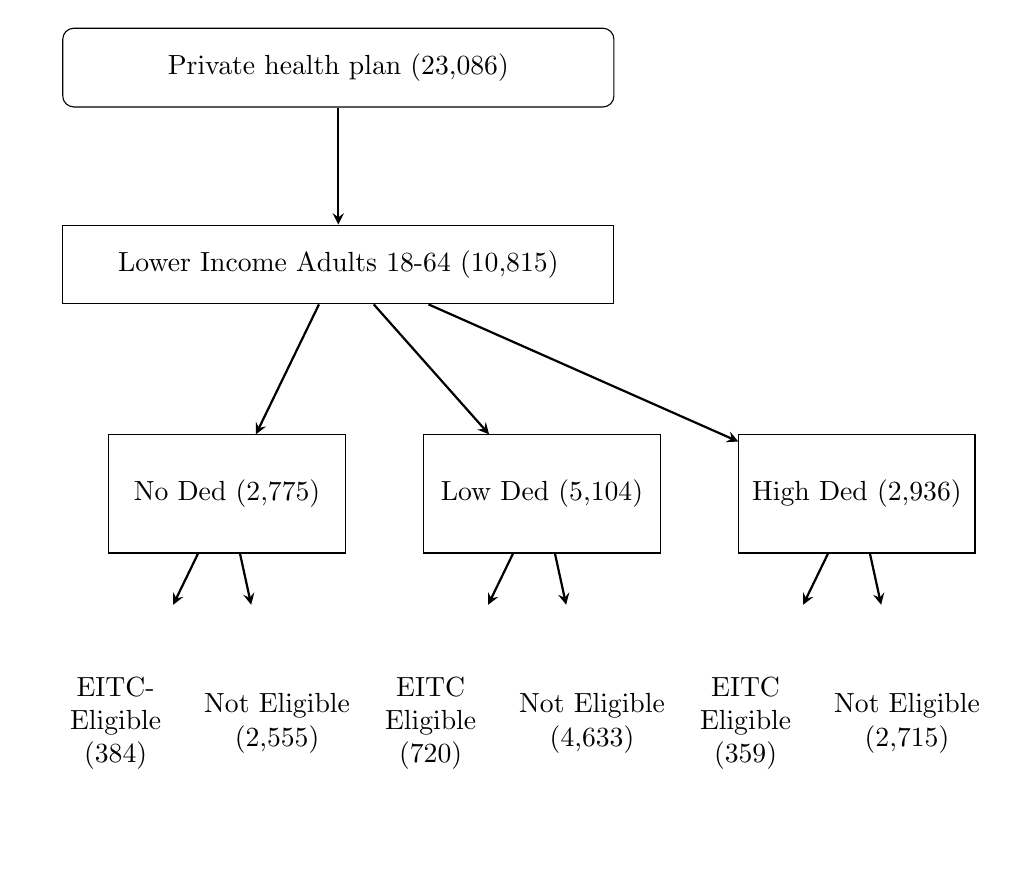
\begin{tikzpicture}[node distance=2cm, scale=0.3]
 

\node [anchor=center] (start) [startstop] {Private health plan (23,086)};
\coordinate[below of=start] (c);
\node (in1)        [process, below of=start, yshift=-0.5cm] {Lower Income Adults  18-64 (10,815)};
\node (noded)  [decision, below left of =in1,yshift=-1.5cm] {No Ded (2,775)}; 
\node (lowded)  [decision,  right of =noded,xshift=2cm] {Low Ded (5,104)};
\node (HDHP)  [decision, right of =lowded,xshift=2cm] {High Ded  (2,936)};
\node (EITC_no)     [EITC, below left of =noded,yshift=-1.5cm] { EITC-Eligible  (384)};
\node (NOEITC_no)     [EITC, right of=EITC_no,xshift=.05cm] {Not Eligible  (2,555)};
\node (EITC_low)     [EITC, below left of =lowded,yshift=-1.5cm] { EITC Eligible  (720)};
\node (NOEITC_low)     [EITC, right of=EITC_low,xshift=.05cm] {Not Eligible  (4,633)};
\node (EITC_high)     [EITC, below left of =HDHP,yshift=-1.5cm] { EITC Eligible  (359)};
\node (NOEITC_high)     [EITC, right of=EITC_high,xshift=.05cm] {Not Eligible  (2,715)};


\draw [arrow] (start) -- (in1);
%\draw [arrow] (in1) -- (pro1);

\draw [arrow] (in1) -- (noded);
\draw [arrow] (in1) -- (lowded);
%\draw [arrow] (pro2) -- (noHSA);
\draw [arrow] (in1) -- (HDHP);

\draw [arrow] (lowded)-- (EITC_low) ;
\draw [arrow] (lowded)-- (NOEITC_low) ;

\draw [arrow] (noded)-- (EITC_no) ;
\draw [arrow] (noded)-- (NOEITC_no) ;

\draw [arrow] (HDHP)-- (EITC_high) ;
\draw [arrow] (HDHP)-- (NOEITC_high) ;

\end{tikzpicture}
 
\end{center}

 	\begin{minipage}{15cm}
		\footnotesize
The units of observations are individuals. The third tier of the sample diagram indicates individual's health plan deductible.
	\end{minipage}

\end{figure}

\FloatBarrier
\subsection{Monthly Health Spending}
To investigate timing of health care consumption within the  months EITC is received, the outcome variable of interest is an individual's total monthly out-of-pocket expenditure.  Health care expenditures, especially at the monthly level, have two unique statistical features. The distribution of out-of-pocket expenditure is skewed and a considerable number of person-months have zero out-of-pocket expenditures. These two statistical features of skewness and mass at zero pose potential challenges \citep{deb_modeling_2018, grafova_how_2020}. Therefore, monthly health expenditures are estimated using OLS and a second approach, using a two-part model (logit and GLM) specification is shown in the appendix as a robustness check of any bias due to the high degree of skewness in the monthly out-of-pocket spending data.
% HOW to inlude a graphic ( PNG) 
\begin{figure}
    \centering 
 \includegraphics[scale=.3]{Monthly_line.png} 
    \caption{Descriptives of Average Monthly Out-of-Pocket (OOP) Health Expenditure}\label{Fig2}
    	\begin{minipage}{15cm}
		\footnotesize
 Shows average total out-of-pocket expenditure in each month. The sample is adults with ESI with annual family income less than \$100,000.  The graph shows the monthly expenditure separately for those adults who do not qualify for EITC and who do not qualify for EITC.
 

	\end{minipage}
\end{figure}
\FloatBarrier




\FloatBarrier



\subsection{Summary Statistics}


Table \ref{Table1} shows detailed demographics of the sample. Column (1) includes all adults with ESI and total household income under \$100,000. Column (2) is further limited to EITC-eligible adults and similarly Column 3 is non-EITC eligible. 

Over 13\% of the lower income privately insured sample are eligible for EITC. The EITC-eligible sample has a higher percentage of lower income adults, which is expected as EITC is means-based program. Importantly, the percentage of adults reporting poor or fair health is comparable across groups. This maybe because this sample is working adults in private health plans. Past work using the NHIS find only small differences in self rated health in an investigation of lower income (collins et al ). 

The EITC sample is younger, another potential reason for similarities in self-rated health. 

The EITC-eligible sample does have a higher percentage of Black and Hispanic individuals than the non-eligible sample.

 Besides having lower income, the EITC-eligible adults demographic characteristics suggests the population may be liquidity constrained.  Empirical evidence shows savings and liquidity vary across age, gender, and race. Younger individuals have had less time to accumulate wealth and savings are more likely to be liquidity constrained \citep{jappelli_who_1990}. 
 Young parents in particular are disproportionately poor compared to other young adult and older parents \citep{carson_poverty_2020}. National surveys also show liquidity differs by race with less than half of black respondents able to cover \$400 expense by cash compared to 71\% of white \citep{federal_reserve_board_update_2020}. In combination the lower income and higher percentage of younger and minority adults suggest the EITC- eligible group may lack liquidity. 

 The average EITC eligibility amount is \$1,861. Given EITC eligibility determination, the average EITC amount increases with number of children. Among individuals with two or more children, the average estimated federal EITC amount is \$2,499. For some households the EITC amount represents a large increase in income. While for others with one or no dependent children the EITC represents a more modest increase in income.



Table \ref{MonthlyTable1} shows detailed monthly health spending by EITC eligibility and the  observations in this table are person months. Column 2 displays months of February and March, when tax refunds are likely received and Column 3 includes all other months. Columns 4 and 5 similarly show descriptives for the non-EITC eligible individuals.
The average monthly spending reveal important trends between the EITC-Eligible and the non-Eligible. On average, the EITC-eligible group has lower total health and out-of-pocket spending than the non-EITC eligible. 

As expected, the EITC-eligible have higher average out-of-pocket spending during the months tax refunds are likely received. 
The EITC-eligible spend (\$20.26) in February and March compared to (\$16.76) in other months. Conversely, the non-eligible spend more consistently over the year. Non-eligible spend (\$25.15) in February and March and \$23.65 in other months. A back of the envelope difference-in-differences estimates produces an increase of slightly over \$2 a month for the eligible in months tax refunds are likely to arrive.  \footnote{$(20.26- 16.76)/ (25.15- 23.65) = \$2.33.$} Of course, many other individual factors which affect care spending, such as age and health plan are not controlled for in this naive estimate. Additionally, the standard errors are large for the monthly spending estimates. 


This trend of higher out-of-pocket spending by the EITC-eligible in the months EITC is received continues for several of the health spending categories. The EITC-eligible spend (\$14.28) a month on office-based care during February and March which is higher than the average spending of (\$9.00) in the non-treatment months.  Office-based visits, are arguably the most discretionary of health care consumption, as they are more easily re-timed compared to inpatient and ER visits. Additionally, office-based visits occur at a much higher rate with over 20\% of months having office-based spending, compared to less than 2\% for outpatient, inpatient and ER spending. Both the discretionary nature and higher rate of occurrence of office- based visits make this care type more likely to be retimed in response to increased liquidity. Overall, the trend of higher average out-of-pocket spending during the months of EITC receipt for the eligible is higher for all health event categories except outpatient and ER.



%%% HOW TO include a table - this is pasted in. (not really recommended) 
\begin{table}[h!]
\centering
\begin{tabular}{l ccccccc}\caption{Characteristics of individuals by EITC- Eligibility}\label{Table1}
%\toprule
%\midrule
&&&& &&&\\
\hline
                    &\multicolumn{2}{c}{(1)}  &\multicolumn{2}{c}{(2)}  &\multicolumn{2}{c}{(3)}  \\
                    &\multicolumn{2}{c}{All}  &\multicolumn{2}{c}{EITC-Eligible}&\multicolumn{2}{c}{Not EITC Eligible}\\
                    &           b&          se&           b&          se&           b&          se\\
\hline
Low-income (200 ppov)&        0.15&        0.01&        0.54&        0.02&        0.10&        0.01\\
Age                 &       41.84&        0.18&       37.62&        0.35&       42.32&        0.19\\
Female              &        0.52&        0.00&        0.54&        0.01&        0.51&        0.01\\
Number of children  &        0.68&        0.02&        1.68&        0.05&        0.56&        0.02\\
College 1yr+        &        0.63&        0.01&        0.51&        0.02&        0.65&        0.01\\
Married             &        0.55&        0.01&        0.56&        0.02&        0.55&        0.01\\
White               &        0.58&        0.01&        0.44&        0.03&        0.60&        0.01\\
Black               &        0.09&        0.01&        0.14&        0.01&        0.09&        0.00\\
Latinx              &        0.10&        0.01&        0.18&        0.01&        0.09&        0.01\\
Poor-Fair Phys Hlth&        0.08&        0.00&        0.09&        0.01&        0.08&        0.00\\
Poor-Fair Ment Hlth &        0.05&        0.00&        0.04&        0.01&        0.05&        0.00\\
EITC amount         &      191.31&       10.80&     1861.48&       67.87&        0.00&           .\\
Northeast           &        0.16&        0.01&        0.13&        0.02&        0.17&        0.01\\
Midwest             &        0.25&        0.01&        0.25&        0.02&        0.25&        0.01\\
South               &        0.37&        0.01&        0.40&        0.03&        0.37&        0.01\\
West                &        0.21&        0.01&        0.22&        0.02&        0.21&        0.01\\
\textbf{Deductible} &&&&&\\
No                  &        0.22&        0.01&        0.22&        0.02&        0.22&        0.01\\
Low                 &        0.49&        0.01&        0.50&        0.02&        0.49&        0.01\\
High                &        0.29&        0.01&        0.28&        0.02&        0.29&        0.01\\
\hline
N               &       10815&            &        1463&            &        9352&            \\

\hline
\end{tabular}
	\begin{minipage}{15cm}
		\footnotesize
Column (1) includes all adults ages 18 to 64 with annual family income under \$100,000 and ESI.  Column (2) is restricted to adults eligible for EITC. Column (3) includes those non-eligible for EITC. 
	\end{minipage}
\end{table}

\begin{table}[h!]
\centering
\begin{tabular}{l cccccccccc}\caption{Characteristics of monthly spending by EITC- Eligibility}\label{MonthlyTable1}
%\toprule
%\midrule
&&&& &&&&&&\\
\hline
   &\multicolumn{2}{c}{Full Sample}    &\multicolumn{4}{c}{\textbf{EITC-Eligible}}&\multicolumn{4}{c}{\textbf{Not EITC Eligible}}\\
                           &\multicolumn{2}{c}{(1)}  &\multicolumn{2}{c}{(2)}  &\multicolumn{2}{c}{(3)}  &\multicolumn{2}{c}{(4)}  &\multicolumn{2}{c}{(5)} \\
   &\multicolumn{2}{c}{All Months}    &\multicolumn{2}{c}{Feb/March}&\multicolumn{2}{c}{Other months}&\multicolumn{2}{c}{Feb/March}&\multicolumn{2}{c}{Other months}\\
                    &           b&          se&           b&          se&           b&          se&           b&          se&           b&          se\\
\hline
\textbf{Monthly Expenditure} &&&&&&&&\\
Total  &      276.04&       16.12&      152.95&       32.33&      179.07&       18.41&      250.34&       35.92&      295.11&       19.94\\
Office-based  &       94.96&        3.67&       67.84&       11.88&       67.28&        8.00&       94.00&        5.72&       98.94&        4.35\\
Outpatient &       50.68&        5.36&       26.80&       13.61&       34.50&        7.12&       42.71&        8.45&       54.67&        7.14\\
 Inpatient  &      112.23&       13.58&       41.67&       26.80&       58.88&       13.01&       98.08&       33.02&      122.79&       16.30\\
 ER       &       18.17&        1.77&       16.63&        5.88&       18.42&        2.24&       15.54&        2.49&       18.71&        2.19\\
 
 \textbf{Monthly Out-of-pocket} &&&&&&&&\\
Total &       23.22&        0.77&       20.26&        4.12&       16.76&        2.34&       25.15&        1.83&       23.65&        0.82\\
Office-based   &       15.55&        0.58&       14.28&        3.65&        9.00&        0.77&       18.01&        1.50&       15.83&        0.61\\
Outpatient  &        3.23&        0.27&        2.08&        1.20&        4.37&        2.00&        2.52&        0.43&        3.26&        0.26\\
 Inpatient   &        2.91&        0.34&        2.89&        1.22&        2.08&        0.53&        3.15&        0.98&        2.96&        0.37\\
 ER     &        1.54&        0.13&        1.01&        0.63&        1.31&        0.32&        1.46&        0.38&        1.59&        0.15\\

\textbf{Percent with Any} &&&&&&&&\\
\textbf{Monthly Expenditure} &&&&&&&&\\
Total &       0.234&       0.003&       0.179&       0.010&       0.190&       0.008&       0.233&       0.005&       0.241&       0.004\\
Office-based &       0.220&       0.003&       0.164&       0.010&       0.175&       0.008&       0.220&       0.005&       0.226&       0.004\\
Outpatient&       0.022&       0.001&       0.017&       0.003&       0.016&       0.002&       0.020&       0.002&       0.023&       0.001\\
Inpatient&       0.005&       0.000&       0.003&       0.001&       0.004&       0.001&       0.005&       0.001&       0.006&       0.000\\
ER&       0.010&       0.000&       0.012&       0.003&       0.013&       0.001&       0.008&       0.001&       0.010&       0.000\\
\textbf{Percent with Any} &&&&&&&&\\
\textbf{Monthly Out-of-Pocket  Spending} &&&&&&&&\\
Total &       0.178&       0.003&       0.132&       0.010&       0.136&       0.007&       0.183&       0.004&       0.183&       0.003\\
Office-based &       0.169&       0.003&       0.123&       0.009&       0.128&       0.006&       0.174&       0.004&       0.173&       0.003\\
Outpatient &       0.011&       0.001&       0.007&       0.002&       0.007&       0.001&       0.010&       0.001&       0.012&       0.001\\
Inpatient&       0.003&       0.000&       0.002&       0.001&       0.003&       0.000&       0.004&       0.001&       0.003&       0.000\\
ER &       0.005&       0.000&       0.004&       0.002&       0.005&       0.001&       0.005&       0.001&       0.006&       0.000\\
\hline
N             &      129780&            &        2926&            &       14630&            &       18704&            &       93520&            \\
\end{tabular}

	\begin{minipage}{15cm}
		\footnotesize
The sample is all person months for adults ages 18 to 64 with annual family income under \$100,000 and ESI. Sample 2 and 3 are person months for adults Eligible for EITC. Sample 4 and 5 are person months non-eligible for EITC. 
	\end{minipage}
\end{table}







\newpage





\FloatBarrier
\section{Methods}


\FloatBarrier
 

%The model investigates monthly health care spending when liquidity constraints are lessened due to an exogenous change in transitory income. 

The federal EITC provides low-income workers with large amounts of liquidity in February and March \citep{mendenhall_role_2012, hamad_short-term_2019}, early in health plans coverage period.
 The following specification examines how the increase in liquidity from the EITC affects those in all private health plans. Note that EITC take up is not directly observed; the estimates are for \textit{eligibility} for the EITC based on individual characteristics, including income, household size and marital status. 

%HOW TO INCLUDE EQUATION
The following specification allows for the comparison of total monthly out-of-pocket health spending  in February and March to all other months of the year for those eligible for EITC compare to those who are not eligible:
\begin{equation}
Y_{it} =  \beta_{1}EITC_{i} +\beta_{2}FebMarch_{t} +\beta_{3}FebMarch_{t}*EITC_{i} + 
 \beta_{4}Year + X_{it}+\varepsilon_{it}  \label{eq:1} 
\end{equation}
where $Y \in \{\text{out-of-pocket expenditure}\}$ for individual $i$ in month $t$.



The variable $EITC_{i}$ indicates whether the individual is EITC-eligible and controls for time invariant characteristics of the EITC-eligible individuals. The variable $FebMarch_{t}$ is equal to one if the month was February or March. The parameter of interest is $\beta_{3}$ which is the difference-in-differences  interaction of the person being EITC-eligible and the month being February or March. The coefficient of interest displays whether the EITC-eligible increase or decrease health spending during the months tax-refunds are likely to arrive. The interpretation of the coefficient is in dollars per month. The variation in this model comes from comparing EITC- eligible individual's spending in February and March to spending in other times of the year. 

%In the first model investigates EITC-eligible individuals response to federal income tax refunds on total out-of-pocket monthly health care spending. This model uses the full sample of lower-income adults.
 The DD strategy compares the monthly health spending of the EITC-eligible to the non-eligible during the treatment months of February and March and compares to the non-treatment months. This identification strategy controls for any secular trends in spending during February or March. February and March likely have different spending averages due to multiple factors such as being early in the calender year and early in the insurance coverage period. The DD controls for these secular trends by using the spending by the non-eligible during this time period as control. This DD empirical strategy has been used in past research of the EITC \citep{hamad_short-term_2019, rehkopf_short-term_2014, hamad_estimating_2018, collin_short-term_2020}.
 
  The vector of person level controls, $X_{it}$ includes: race (White, Black , Latinx, or other), health status (1=poor or fair), mental health status (1=poor or fair), marriage status (1=married), poor(1=$<$ 200\% poverty line), age, age squared, age cubed, number of people in the household, number of children in the household, education level (1= some college), plan deductible (1=no , 2=low, 3=high), month, region (North, South, East, West) and year fixed effects (2011 - 2016). The individual level controls capture any observable characteristics that are associated with health expenditure. Estimates are weighted using MEPS sampling weights and the standard errors are clustered at the primary sampling unit to account for the complex survey sampling design. 

Next, health spending is modeled separately, for each category of:  office-based, inpatient, outpatient and emergency room.  Investigation of health spending by care type provides insight into whether individuals respond to liquidity for a particular spending category. It is hypothesized discretionary care such as office-based visits will be the most sensitive to the increased income for multiple reseasons. First, office-based care is more easily re-timed. Second, the consumption smoothing literature suggests health spending that is viewed as in investment (i.e preventive care) are more likely to be forgone when households experience an economic shock.  Research shows these types of visits are forgone for vulnerable populations \citep{sherman_health_2017} .

Then, the association between EITC recipient and total health spending is investigated separately by health plan enrollment. This specification shows whether individuals with higher deductibles are more or less liquidity sensitive during tax filing months. Given the conceptual model of liquidity sensitivity adults with higher deductibles are expected to have the largest effects \cite{gross_liquidity_2020}.


To investigate whether EITC amount is associated with increased care during the treatment months the model is restricted to those receiving EITC, having more than one child. This provides a test to investigate if EITC is effecting those who qualify for a higher amount. Heterogeneous effects are estimated separately for racial sub-groups. 





\section{Findings}

The results in Table \ref{table3} show the effect of EITC receipt on out-of-pocket health expenditure using Equation \ref{eq:1}. Panel A includes all lower income adults. The dependent variable in Column (1) is total monthly out-of-pocket expenditure. The estimates on February or March indicate slightly lower spending in the months tax refunds are likely to arrive. This lower out-of-pocket spending is expected as the spot prices of care are generally higher during the early months of the calendar year. The negative direction of the estimates suggests adults may reduce spending in the period before they have full benefits of their health plan \citep{brot-goldberg_what_2017}.

EITC- eligibility is associated with  -\$2.96 (p < 0.01) less monthly out-of-pocket expenditure. Eligible adults are spending less on health care despite having similar health status to non-eligible, as displayed in Table \ref{MonthlyTable1}. Compared to the monthly average spending of \$19, EITC-eligible spend 15\% less. The considerable difference in spending suggests EITC-eligible face financial difficultly in affording out-of-pocket health costs. This aligns with the predictions that EITC-eligible, after controlling for income and health status have lower levels of out-of-pocket spending.


The estimate of interest is the different-in-differences interaction of Feb or March x EITC-eligible. For the sample of lower income adults, the estimate of \$0.03 (p>0.10) is small, positive and insignificant.  This estimate indicates being eligible for EITC is not significantly impacting out-of-pocket health spending during the months it is received. 

Some health care is more likely to be re-timed in response to the increased liquidity. The most discretionary type of care are office-based visits, which often include preventive care, screenings and chronic disease management. Conversely, emergency room visits often occur when pressing health needs arise. Columns (2)-(5) estimate Equation \ref{eq:1} separately for each of the health event categories. Office-based out-of-pocket spending is \$1.41 (p<0.10) less during the early months of the year. EITC-eligible adults spend  \$2.37 (p<0.01) less on office-based out-of-pocket care.  The significantly lower office-based spending for EITC- eligible align with the expectation that discretionary care is responsive to ability to pay.  Similarly, as predicted, the DD estimate shows positive effects of the tax receipt for the EITC-eligible in the months it is received. The increase of about \$.20 a month is small when compared to the average monthly office-based spending of \$19. The increased liquidity EITC provides does not significantly influence office-based spending for the eligible.
%Office-based health expenditure is arguably the most discretionary of the health spending categories, meaning adults are able to schedule and time office-based visits if they cannot pay the out-of-pocket costs.

The DD estimates for the health spending categories of outpatient and inpatient are negative and insignificant. The results for these spending categories are expected as these health care visits are less discretionary and adults are less likely to time these visits based on ability to pay. 

For ER visits, spending is about 50\% lower in February and March, compared to other months of the year. EITC-eligible spend \$.14 (p>0.10) more a month on ER visits compared to the non-eligible. The slightly higher ER spending, in combination with significantly lower office-based, suggests sub-optimal health care seeking for the EITC-eligible. Findings are similar to those of \cite{sherman_health_2017} who found the lower income adults with ESI have the lowest rates of preventive care which results in higher emergency spending. The DD estimate for ER spending is positive but non-significant. Overall, in the full sample of lower income adults there is no significant increase in spending during the months tax refunds are likely to arrive. This maybe because a portion of the lower income adults sample has public insurance and are not facing the high cost sharing requirements of employer sponsored health plans.
 
Panel B includes the population of interest, lower income working adults with ESI.
When adults with public health insurance are removed from the sub-population (Panel B), the estimates increase in size and in the expected direction.  The estimates on February and March are negative and significant for total, office-based and outpatient out-of-pocket spending.  The  lower spending in the early months of the year are expected, as 75\% of the ESI sample has some level of cost sharing. Adults are likely paying the full out-of-pocket cost for care in first months of the year as they likely have not reached the deductible. Spending \$5.30 (p<0.05) less a month early in the year indicates cost sensitivity to spot prices of care.  EITC-eligible have lower total out-of-pocket monthly spending compared to the non-eligible. The DD estimate for total out-of-pocket spending is positive although the estimated \$2 increase in monthly spending is economically and statistically insignificant, compared to the average monthly spending of \$23.   \footnote{given an N=21,630 person months in the treatment period, a mean outcome of 20.90 and a SD of 160.57, The minimum detectable effect (MDE) for this is \$9.21 at a power of 80.}

For office-based spending, there is indication of both sensitivity to price and ability to pay. For adults with ESI, average office-based spending is significantly lower in February and March and adults EITC-eligible adults are spending significantly less compare to the non-eligible. The DD estimate shows an increase \$3.10 (p>0.10) a month for the EITC- eligible during tax months. As expected, the effect of liquidity is largest for office-based care compared to outpatient, inpatient and ER spending categories. 

 For adults with ESI, the average monthly health spending differs widely by spending category. Office-based care has the highest average spending at \$16 per month. Comparatively, outpatient, inpatient and ER spending have monthly averages of \$3 or less. The larger size of the DD estimates for the discretionary care are consistent with apriori expectation of which care is likely to be influence by the increase in liquidity. The DD estimates are as expected, with positive coefficient on the interaction, but noisy. This noise is due to the fact levels of spending are low per month since a large portion of adults have \$0. Overall, findings shows no major increase among EITC-eligible during tax refunds.  


\subsection{Effects by Deductible Level}
Table \ref{table3} Panels C and D show the effects among lower income adults with low and high deductible levels of cost sharing. Although the overall estimates do not show strong patterns, there is likely a heterogeneous response to the EITC for subgroups.  Several of the findings align with past research that lower cost sharing provide smoother health care consumption \citep{ericson_liquidity_2018}.

First of all, for adults in low deductible plans, the difference between spending in the early months of the year compared to other months of the year is small (Panel C). The estimate of only \$1.67 (p>0.10) less spending in February or March provides evidence of consistent within- year out-of-pocket spending. For liquidity constrained adults, the lower out-of-pocket spending necessary before full insurance starts may provide the ability to seek care when needed instead of delaying until deductible is reached.
Second, EITC-eligible adults in low deductible plans spend more out-of-pocket compared to the non-eligible. This higher spending by the EITC- eligible only appears among adults in low deductible health plans.  Third, there is no significant change in total out-of-pocket spending during the months EITC is received for the eligible, as indicated by the DD estimate of -\$.51 (p>0.10). As predicted by the \cite{gross_liquidity_2020} model, adults in low deductible plans show little sensitivity to the liquidity EITC provides.
 
In column 2 of Panel C, estimates for office-based care show lower spending in the early months of the year. The magnitude and significance of the estimate is similar to that of the full lower income sample. This negative estimate likely arises because low deductible plans still require out-of-pocket expenditure. EITC-eligible have similar average office-based care spending compared to non-eligible. As predicted the DD estimate for office-based care is small in magnitude and positive for adults facing lower cost sharing. 
 
 For the other health spending categories, there is no indication of within - year timing of care. This is again expected as outpatient, inpatient and ER visits tend to be purchased when the care is necessary as opposed to delaying until the deductible is reached. EITC-eligible in low deductible plans spend similar amounts out-of-pocket compared to non-eligible on outpatient, inpatient and ER. The DD estimates for adults in low deductible plans show small and negative responses to the liquidity. 
 Overall, the direction and size of the estimates indicate low deductible plans may allow adults to consume care when necessary, as opposed to timing care when spot prices are lower or when liquidity arrives. 


Panel D shows results for adults facing the highest levels of cost sharing, those in HDHPs. In February and March, out-of-pocket spending is lower in all health categories and significantly lower for total and outpatient spending. The lower spending during periods of high spot prices align research which found deductibles influence the within year timing of health care \citep{gerfin_healthcare_2015, lin_intertemporal_2019, cabral_claim_2017, brot-goldberg_what_2017}.  Adults in HDHPs spend about 45 \% less in early months of the year, an economically significant reduction in spending . 
Comparably, \citep{brot-goldberg_what_2017} found a 42\% reduction spending before the deductible in a sample of high income adults in HDHPs. This indication of timing of care among lower income adults is concerning as delaying of care can lead to adverse health outcomes if necessary or preventive care is delayed.
 The lower spending during higher price periods and for financially vulnerable populations suggests cost sharing features may influence health care seeking among adults in HDHPs. EITC-eligible adults in HDHPs spend \$11.49 (p<0.01) less monthly out-of-pocket. Compared to the average monthly spending of \$32, the EITC-eligible are spending 37\% less than the non-eligible. The DD estimate is large, with over a \$9 increase in out-of-pocket expenditure,  but the standard error makes the estimate imprecise. Therefore, one is not able to reject the null hypothesis that there was no short-term effect of EITC refund in February or March on out-of-pocket spending. 

The effects on total health spending appear to be driven by discretionary, office-based spending shown in (Column 2). Lower office-based spending is seen early in the year and EITC- eligible are spending \$5.74 (p<0.05) less a month compared to the non-eligible. The effect of EITC receipt is large with a \$9 increase in office-based out-of-pocket spending during tax receipt months. Smaller DD estimates are seen for outpatient, inpatient and ER and is likely due to the increased difficultly to time these visits. 
  
  The positive direction of the DD estimates for total and office-based spending among adults in HDHP's align with the predictions of the conceptual model. Those facing the highest prices have larger spending increases during times of increased liquidity. Although not significant, the large estimates for adults in HDHPs, indicate the tax refunds may allow for the purchasing of care which was otherwise delayed or forgone.

Overall, the heterogeneous effects by level cost sharing are in the direction that the \cite{gross_liquidity_2020} conceptual model predicted. Adults in low deductible plans have smaller within year timing effects, suggesting low deductible plans allow for purchasing of care when needed, and not when it is lower priced or when income arrives. Among those in low deductible plans, the financially vulnerable population spend on average more than the non-EITC eligible. 

For those facing high out-of-pocket prices, larger and concerning effects are seen. Significantly lower spending by the EITC-eligible in HDHPs may, as past work has shown, indicate out-of-pocket costs are impacting care seeking for financially vulnerable \citep{haviland_how_2011}. 

The DD estimates are as expected  positive, with noisy coefficient on the interaction. Overall, findings shows no major increase in out-of-pocket spending among EITC-eligible during time of tax refunds. The size of results are similar to \cite{hamad_short-term_2019} who found a non-significant change in out-of-pocket spending of \$0.67 per \$1,000 of EITC and \$-0.14 for adults enrolled in private health insurance for adults in older data. \footnote{Private health insurance includes but is not limited to insurance through an employer.} \cite{hamad_short-term_2019} additionally did not control for cost sharing in the model. The two-part model to account for skewness of health care data are shown in the Appendix and reveals similar results.


\begin{table}[h!] \caption{Monthly Out-of-Pocket Health Spending} \label{table3}
  \centering {

\estwide{EITCm1_ALLPEOPLE_private_V1.tex}{5}{c}
}
	\begin{minipage}{15cm}
		\footnotesize

Results show estimates from Equation \ref{eq:1}. Observations are person months.  In Column (1) the outcome variable is total monthly out-of-pocket spending. In Columns (2)-(5) the outcomes are each of the health spending categories separately.  In Panel (A) the sample is adults with family income under \$100,000.
In Panel (B) the sample is adults with family income under \$100,000 and employer sponsored health insurance. Panel (C) includes lower income adults with low deductible and panel (D) includes lower income adults with high deductible plans. All models include the following controls:  race (White, Black , Latinx, or other), health status (1=poor or fair), mental health status (1=poor or fair), marriage status (1=married), poor(1=$<$ 200\% poverty line), age, age squared, age cubed, household size, number of children, education level (1= at least some college), plan deductible (1=no , 2=low, 3=high), month, region (North, South, East, West), and year fixed effects (2011 - 2016). Estimates are weighted and standard errors are clustered at the primary sampling unit (PSU) level to account for MEPS’ complex survey design. * $p<0.10$, ** $p<0.05$, ***$ p<0.01$
	\end{minipage}
\end{table}
















\section{Conclusion}

 A recent policy brief coined the term ``deductible relief day" or the day by which average spending for people with ESI is enough to reach the average deductible \citep{lee_deductible_2019}.   In 2006,  ``deductible relief day" was February 28th. In 2019, as deductibles increased, it was May 19th. The lump sum payment EITC arrives in a period of financial vulnerability and may assist people with employer sponsored ESI who are in a period before they have full benefits of their health plan \citep{lee_deductible_2019}.


Rising out-of-pocket costs and delaying of care in response can impact household's members health and financial well-being. This study investigates one mechanism which may facilitate expenditures: predicted short term liquidity. Across estimates it appears there is a  positive trend in health care spending around the time EITC payments are received among people who are eligible, but these estimates are imprecise and not statistically significant.    These estimates tend to be larger for low income adults with higher deductible plans. The spending effects of the EITC are also mainly observed for office-based and outpatient care, which are more discretionary than emergency room visits, for example. This is important, especially since low-income workers have lower rates of preventive care and highest emergency room visits  \citep{sherman_health_2017} . 

EITC-eligible adults have many other consumption demands on their tax refund.  Moreover, the EITC may not be enough to cover the high spot prices costs of health care  \citep{claxton_employer_2018}.  Also, consumers who are aware that the refunds will arrive early in the year  may purchase health care when it is necessary and pay the bills when income arrives. 

Liquidity is not directly observed in the data. These estimates are based on an inferred effect of liquidity for the adults who are EITC-eligible. This results in downward biased estimates of the effects of the tax refunds as there may not be enough of an increase in spending for liquidity constrained adults to reveal an effect relative to those who are non-liquidity constrained.  


In the investigation of heterogeneous differences to the increases to income across race again no significant increase is seen across different groups who are likely liquidity sensitive. Although for black populations the EITC-eligible are spending significantly less than the non-eligible indicating reduced amount of care and positive effects are seen during months of tax receipt. Despite the imprecise estimates, the direction and size for black adults are expected, although concerning.  Racial disparities in health care exist, and this provides evidence private health plans and costs sharing may adversely impact black populations \citep{charron-chenier_racial_2018, dogra_consumption_2016}.  

Selection into certain health plans may be confounding estimates. Individuals choose health plans based on their expected health care spending and knowledge of their finances. For example, HDHPs are promoted by policymakers as a way to have workers internalize more of the costs of care, resulting in reduced use of care and lower overall costs. But this may only be true for individuals who have both the incentive and ability to monitor their level of health care consumption.   The population of this study is also unique, with a focus on low-wage working adults with employer-sponsored insurance. This is specific to some industries such as in government, manufacturing, educational services and health care \citep{fronstin_how_2020}.  The EITC's work requirements are associated with increased access to private insurance \citep{lenhart_effects_2019,hoynes_income_2015,baughman_evaluating_2005}.  Another consideration is that adults with children may respond to the EITC by increasing their health spending for their children \citep{monheit_how_2020}. The focus of this study is on  health care consumption of adults, but there could be unobserved effects of the EITC on parent's choices to accelerate health care for children which might otherwise be delayed or forgone. 

One policy debate surrounds if the EITC should be converted to periodic payments.  Periodic payments of EITC would lower the volatility in income and smooth consumption.   This study does not offer evidence directly on this point, but if people have other demands on a lump sum payment, it is possible a more graduated monthly payment will spread out that consumption, offering more liquidity for health care consumption.
%The CTC in 2021 also piloted monthly payments. . 

These findings add to the growing literature on health spending and household finance. Past results have varied with some finding increases in health care spending at tax time using aggregated consumption data \citep{parker_consumer_2013, johnson_household_2006, farrell_coping_2017}. Conversely, \cite{hamad_short-term_2019} specifically investigated EITC receipt on health expenditure using the 1997---2012 MEPS and found no change in out-of-pocket health care expenditures. This current study shows that EITC-eligible individuals in HDHPs (which were uncommon in the \cite{hamad_short-term_2019} study era) have higher average health expenditures during the tax filing period, although the estimate was not statistically significant. 

Continued research on consumers' response to cost sharing are important for understanding household finances, health and insurance design. Current policies emphasize liquidity in the form of savings in Flexible Spending Accounts (FSAs) and Health Savings Accounts (HSAs), but these are not widely used, especially among lower income, more wealth constrained households \citep{helmchen_health_2015}. Policymakers and health practitioners may consider ways to help lower-income families to fund and use tax-advantaged health savings accounts, including in conjunction with EITC tax refunds.  Additionally, health policies such as income-based deductible may help to lessen the burden of out-pocket-spending for low income households \citep{sherman_health_2017}.

Policy discussions regarding insurance contracts often focus on providing households risk protection while limiting moral hazard \citep{gross_liquidity_2020}. This view is not taking into account the additional benefit of low-cost sharing insurance for households facing liquidity constraints \citep{ericson_liquidity_2018}. Generous insurance provides these consumers the ability to consume health care when it is needed and not have to delay care until income arrives \citep{gross_liquidity_2020}. This additional advantage of full coverage should be considered in policy design especially for low-income households. 

There are several limitations to this study. First, this not a causal analysis of how deductibles effect health care spending or timing. Health plan choice and EITC eligibility are all endogenous with health status and use of care. These descriptive findings still provide useful evidence, however. Second, employer contributions may drive individuals into higher health care utilization \citep{haviland_how_2011}. However, the MEPS does not differentiate if the plan is associated with an HSA or an HRA, if the HDHPs meet all the requirements for HSAs, or if an employer contributed to these accounts. Fourth, the MEPS does not include all of the health plan choices or sets people choose from in the coverage year. 

Additionally, emergency, outpatient and inpatient visits, unlike office-based visits, often do not necessitate upfront payments, making  expenditures less sensitive to liquidity or income. Also, many preventive services are covered by insurance without consumers facing co-payments or coinsurance. Individuals may be consuming preventive care during office-based visits, but this would not be included in the out-of-pocket data.  On the other hand, these types of preventive visits may lead to subsequent non-covered costs if follow-up examinations, test or procedures are then triggered by these visits.  Future studies could investigate differences by the type of care in periods of increased income--for example more discretionary care such as expensive imaging procedures and prescription drug purchases among working-age adults. 


Past work shows during periods of income reductions and economic downturn single-mother families reduce their own health spending while increasing health expenditure towards their children \citep{monheit_how_2020}. Future research should investigate family level health spending, where this effect may be found to a greater extent. Additional studies could examine within-household allocations of health spending during periods of increased income. Future could investigate variation in state tax laws regarding EITC effect on smaller health items such as drugs and health products among families with children. In addition, drugs and other health products have the feature of having to be paid for at time of receipt whereas health payments for medical visits are often not due when services are received.    


%%% THIS IS HOW TO INCLUDE AN BIBLIOGRAPHY!

\clearpage

\singlespacing
\singlespacing
\bibliography{EITC_liquidity_April27}



\addcontentsline{toc}{section}{Appendices}


\section{Appendix}
\begin{figure}
    \centering
\includegraphics[scale=.3]{Fig3.png}
    \caption{Monthly Health Spending, Adults With ESI}\label{Fig3}
    	\begin{minipage}{15cm}
		\footnotesize
Results show estimates from Table \ref{table3}, Panel B. Observations are person months. 
  Sample includes adults with private insurance and family income less than \$100,000. The first outcome, marked with an "x"  is total of monthly out-of-pocket expenditure. The subsequent outcomes are each of the four expenditure categories separately office-based, outpatient, inpatient, and ER.  All models include the following controls:  race (White, Black , Latinx, or other), health status (1=poor or fair), mental health status (1=poor or fair), marriage status (1=married), poor(1=$<$ 200\% poverty line), age, age squared, age cubed, education level (1= at least some college), plan deductible (1=no , 2=low, 3=high), region fixed effects (North, South, East, West), month, and year fixed effects (2011 - 2016). Estimates are weighted and standard errors are clustered at the primary sampling unit (PSU) level to account for MEPS’ complex survey design.
	\end{minipage}
\end{figure}
\FloatBarrier



\section{Treatment Month Robustness Checks}
\begin{table}[h!] \caption{Robustness Check: Monthly Out-of-Pocket Health Spending} \label{table3_robustnesscheck}
  \centering {

\estwide{EITCm1_ALLPEOPLE_private_APRIL.tex}{5}{c}
}
	\begin{minipage}{15cm}
		\footnotesize

Results show estimates from Equation \ref{eq:1} with the treatment months of February, March and April. Observations are person months.  In Column (1) the outcome variable is total monthly out-of-pocket spending. In Columns (2)-(5) the outcomes are each of the health spending categories separately.  In Panel (A) the sample is adults with family income under \$100,000.
In Panel (B) the sample is adults with family income under \$100,000 and employer sponsored health insurance. Panel (C) includes lower income adults with low deductible and panel (D) includes lower income adults with high deductible plans. All models include the following controls:  race (White, Black , Latinx, or other), health status (1=poor or fair), mental health status (1=poor or fair), marriage status (1=married), poor(1=$<$ 200\% poverty line), age, age squared, age cubed, household size, number of children, education level (1= at least some college), plan deductible (1=no , 2=low, 3=high), month, region (North, South, East, West), and year fixed effects (2011 - 2016). Estimates are weighted and standard errors are clustered at the primary sampling unit (PSU) level to account for MEPS’ complex survey design. * $p<0.10$, ** $p<0.05$, ***$ p<0.01$
	\end{minipage}
\end{table}






\end{document}
